\begin{figure}
\centering
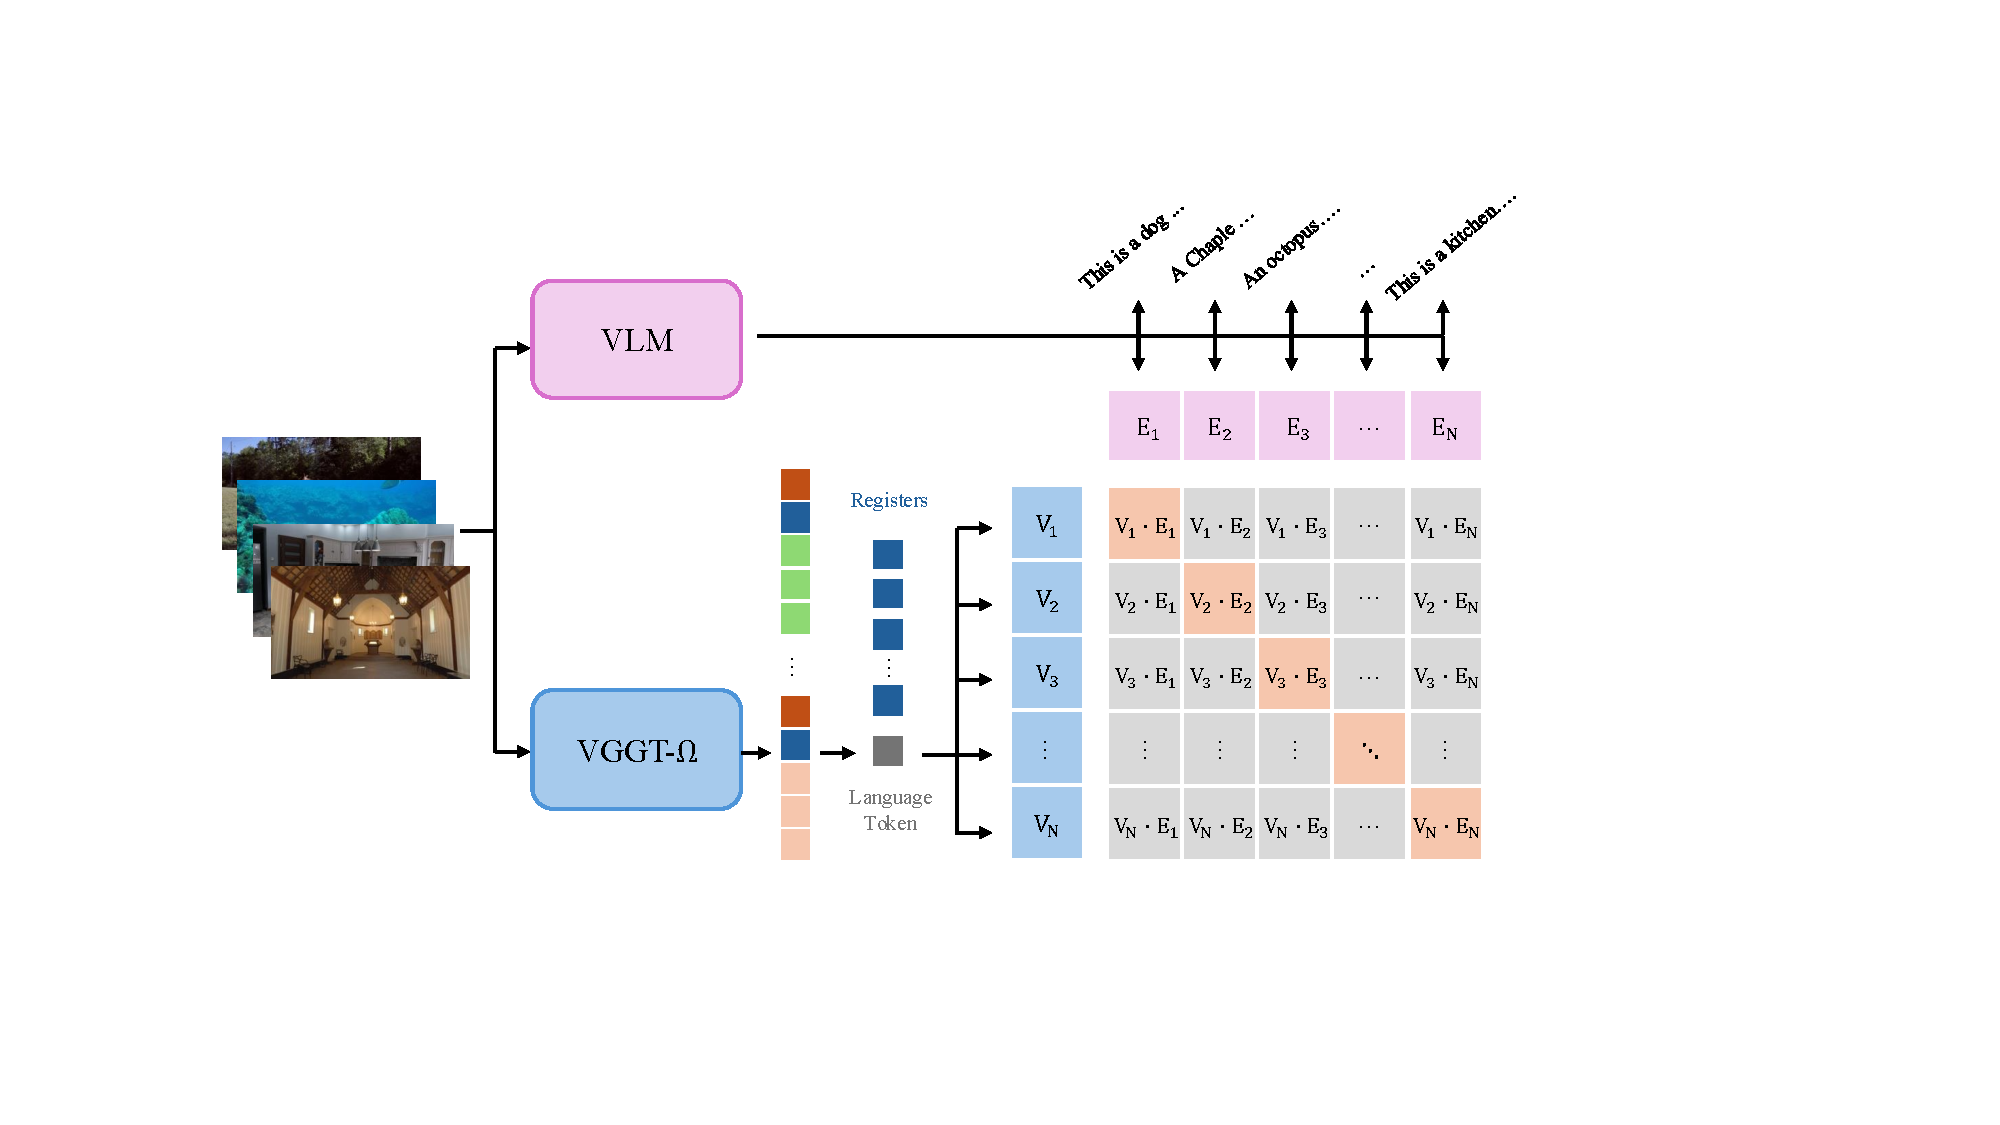
\includegraphics[width=0.95\linewidth]{figures/text_alignment.pdf}
\caption{\textbf{Language Alignment.} 
We conduct language alignment to verify whether the registers contain high-level information. 
For each sequence, a VLM describes the scene content, coarse layout, and appearance, and the generated text tokens are mean-pooled to form the language embedding. 
On the \method side, a small self-attention stack takes the registers and a learnable language token as input, and the output language token is projected to form the register-derived embedding. 
The two embeddings are optimized with a symmetric InfoNCE loss over all sequence-description pairs in the global batch.
}%
\label{fig:text_alignment}
\end{figure}

